\chapter{Optical RFFE Communication}
\label{cha:optical_rffe_comm}
The WiSpry WS1040 digital capacitor is adjusted using the MIPI RFFE (RF Front End) protocol. In order to simplify sweep-measurements, which are a large part of this project, it is advantageous to be able to adjust the capacitance from outside the anechoic chamber. As having a long copper cable from running from the antenna to outside the chamber might disturb the measurement significantly, a fiber optic cable will be used for communication between computer and antenna. As the fiber optic cable contains no metal, it should be less disturbing to the measurements.

The RFFE protocol requires three signals:
\begin{description}
    \item[SDATA] Bi-directional serial data signal carrying ones and zeros from the master (PC) to the slave (ws1040) and back. Both the master and the slave can drive this line.
    \item[SCLK] Serial clock. The master both clocks data to and from the slave.
    \item[VIO] Reference voltage of \SI{1.8}{V}. The SDATA and SCLK signals swing from \SI{0}{V} to VIO so VIO is the common reference -- not ground!
\end{description}
The WS1040 chip is rated for a supply voltage between \SI{2.7}{V} and \SI{5.0}{V}, so the VIO voltage is generated separately for communication.

The purpose of this communication link is solely to write to registers in the WS1040 so only one-way communication is necessary. To minimize the number of fibers, it is chosen to communicate via UART (Universal Asynchronous Receiver/Transmitter) over the fiber and generate the RFFE signals locally on by a microcontroller at the antenna side. This requires only one fiber to be connected. In case a response were required, two fibers could be connected.

\begin{figure}[htbp]
    \centering
    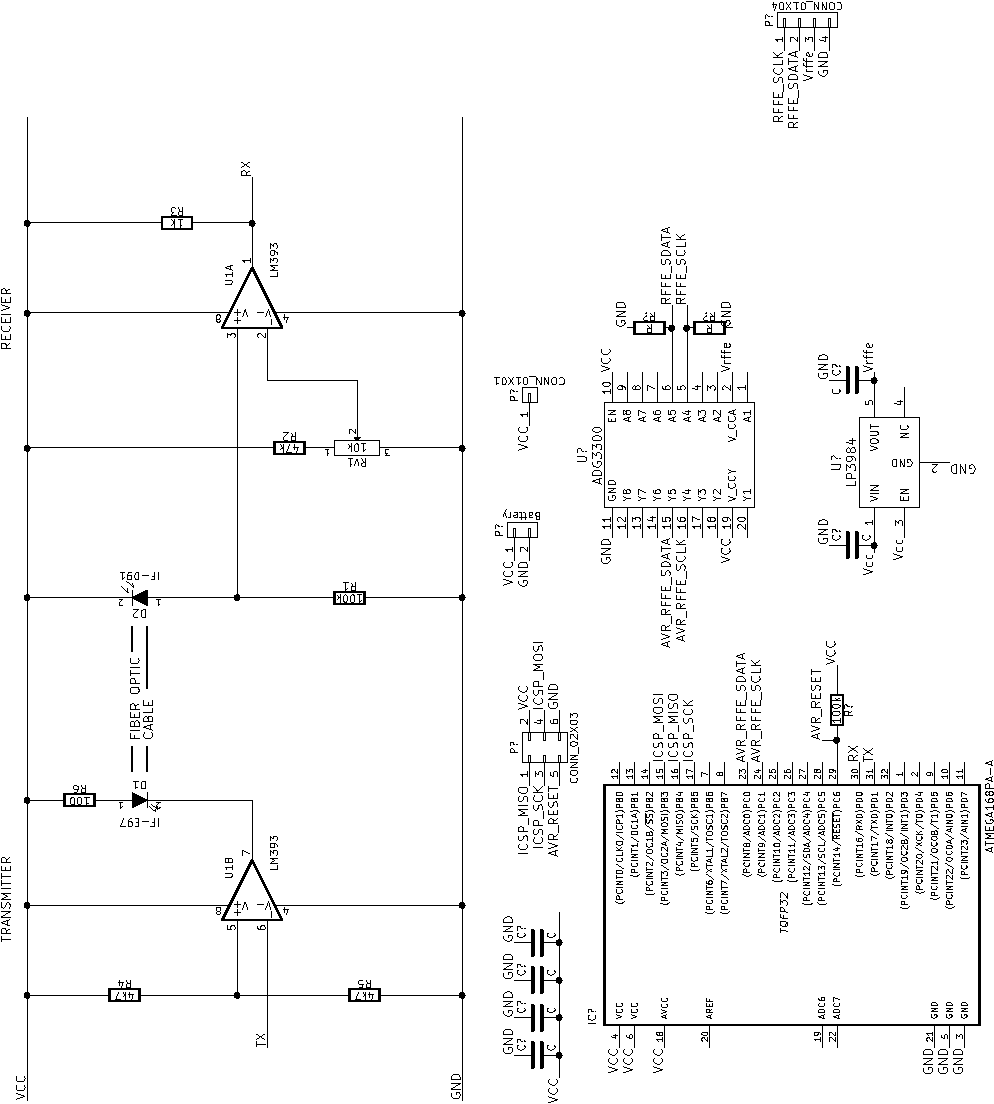
\includegraphics[angle=270, width=\linewidth]{img/optical_rffe/schematic}
    \caption{Schematic for optical RFFE communication -- antenna-side. \fixme{Update schematic: New RFFE pins (PB6=SDATA PB7=SCLK) and annotations on schematic}}
    \label{fig:rffe_schematic}
\end{figure}

The total schematic is shown in Figure~\ref{fig:rffe_schematic}. Both the transmitter and receiver is included on the antenna-side board and the PC-side board. On the PC side, the RX and TX lines are connected to a PC using an USB to UART adapter. On the antenna side, the RFFE\_SCLK, RFFE\_SDATA, and Vrffe lines are connected to the WS1040 chip.

In the following, each part of the design is described.

\section{Transmitter}
The transmitter is made up from an open-collector comparator. The UART TX signal is connected to the inverting input of the comparator and a voltage divider, dividing the supply range in half, is connected to the non-inverting input. This means that when the input-signal is high (above $V_{cc}/2$), the comparator will pull down the cathode of the LED down to ground, lighting up the LED. When the input-signal is low (below $V_{cc}/2$), the output of the comparator will be floating, and no current will run through the LED -- no light.

\section{Receiver}
The light detector (IF-D91) functions as a light-dependent current source. When lit, around \SI{3}{\micro\ampere} is supplied and when dark, around \SI{10}{nA} is supplied. When this current is supplied to a \SI{100}{k\ohm} resistor, the voltage will alter between \SI{300}{mV} (light) and \SI{1}{mV} (dark). The potentiometer on the inverting input of the comparator is used to set a threshold between these two values. By way of the pull-up resistor on the output, this means that the output will be high when light is supplied to the light detector and the output will be low when no light is supplied.

\section{Micro Controller and Protocol}
\fixme{Finish the chapter from here.}

\section{Level Shifting and WS1040 Interface}
